\section{Etherless-cli architecture}
\subsection{The architecture}
The Etherless-cli is the client component that communicates with the AWS applications and the smart contract in the Ethereum\glo network.
This component is made with TypeScript and complied upon execution in Javascript ES6.
The interaction with the program happens through the command-line interface.
At the start of the execution, the program instantiates every class and processes the request made by the user.
To simplify the component, we divided it into two modules, Network Entities, and Command Entities.

\begin{figure}[h]
	\centering
	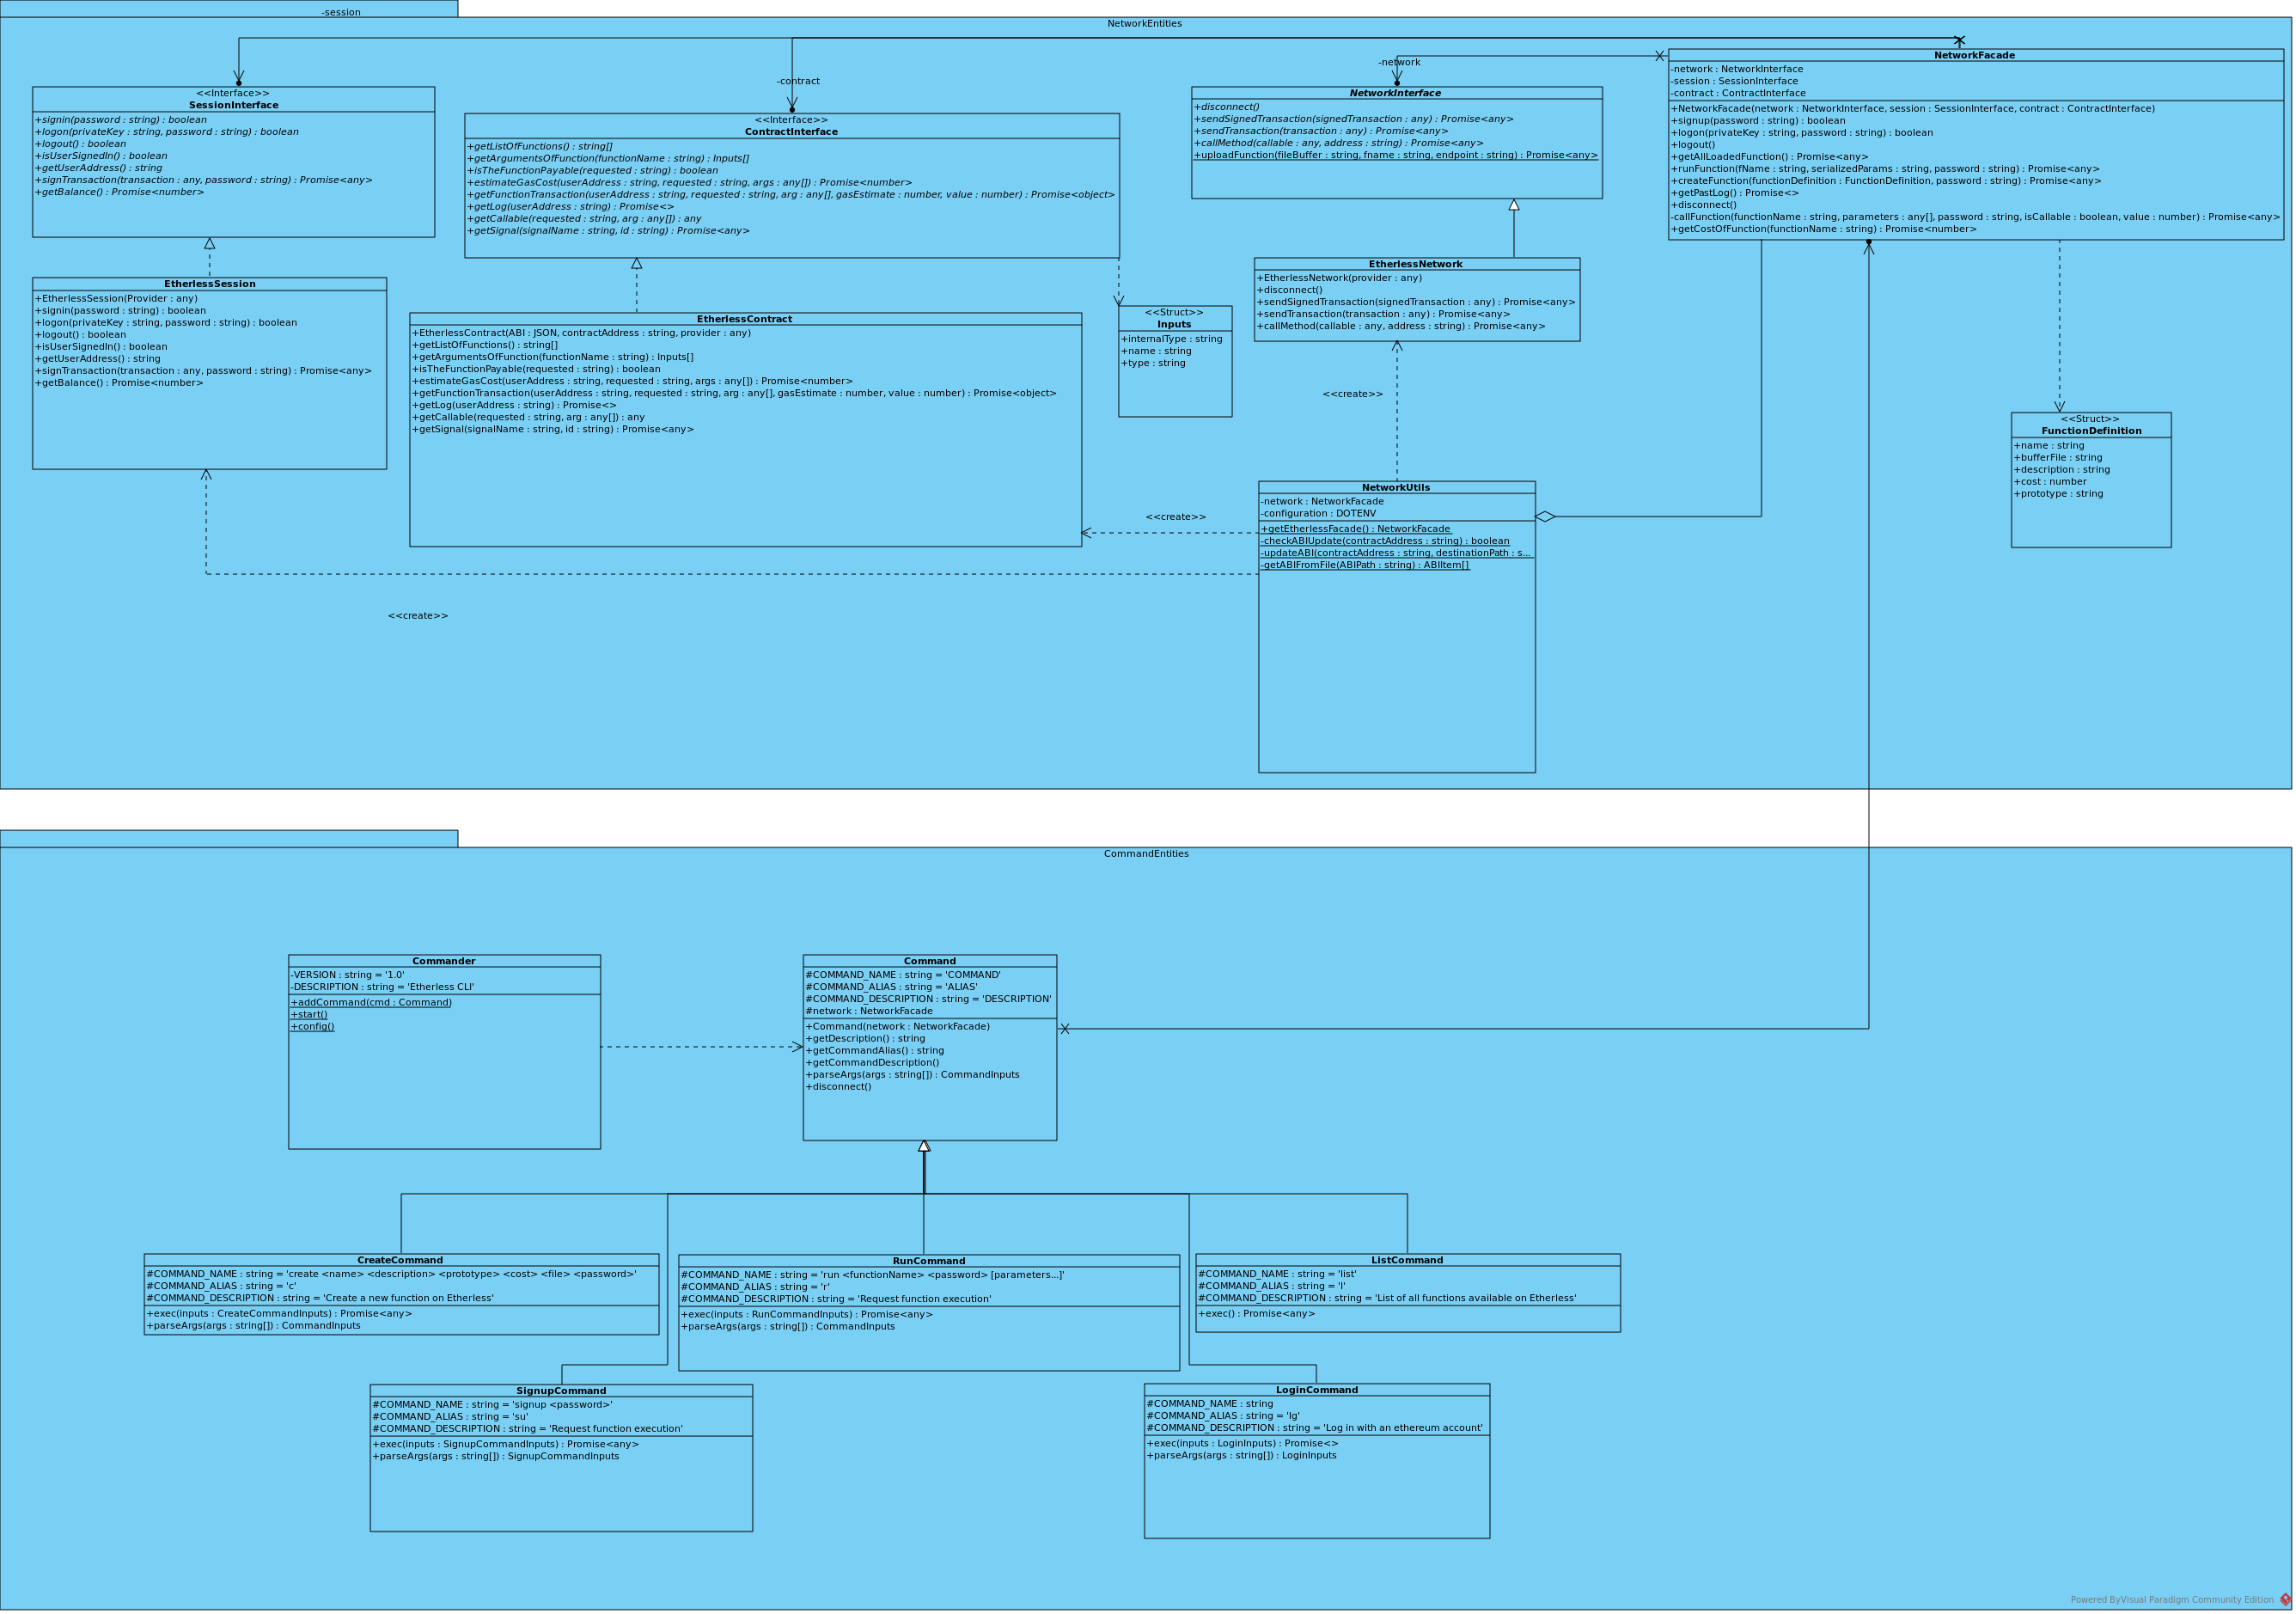
\includegraphics[width=\textwidth]{./res/img/Etherless-cli.png}
	\caption{Architecture overview diagram of Etherless-cli}
\end{figure}

\subsection{The Network Entities}
We designed the architecture of NetworkEntities with interoperability and ease of use in mind.
We based the architecture on a \textbf{facade design pattern} that should expose at the user all the functionalities
of the network through the use of specific interfaces without binding to a specific library for communication
with the Ethereum\glo network.
\subsubsection{Architecture overview}
\begin{figure}[h]
	\centering
	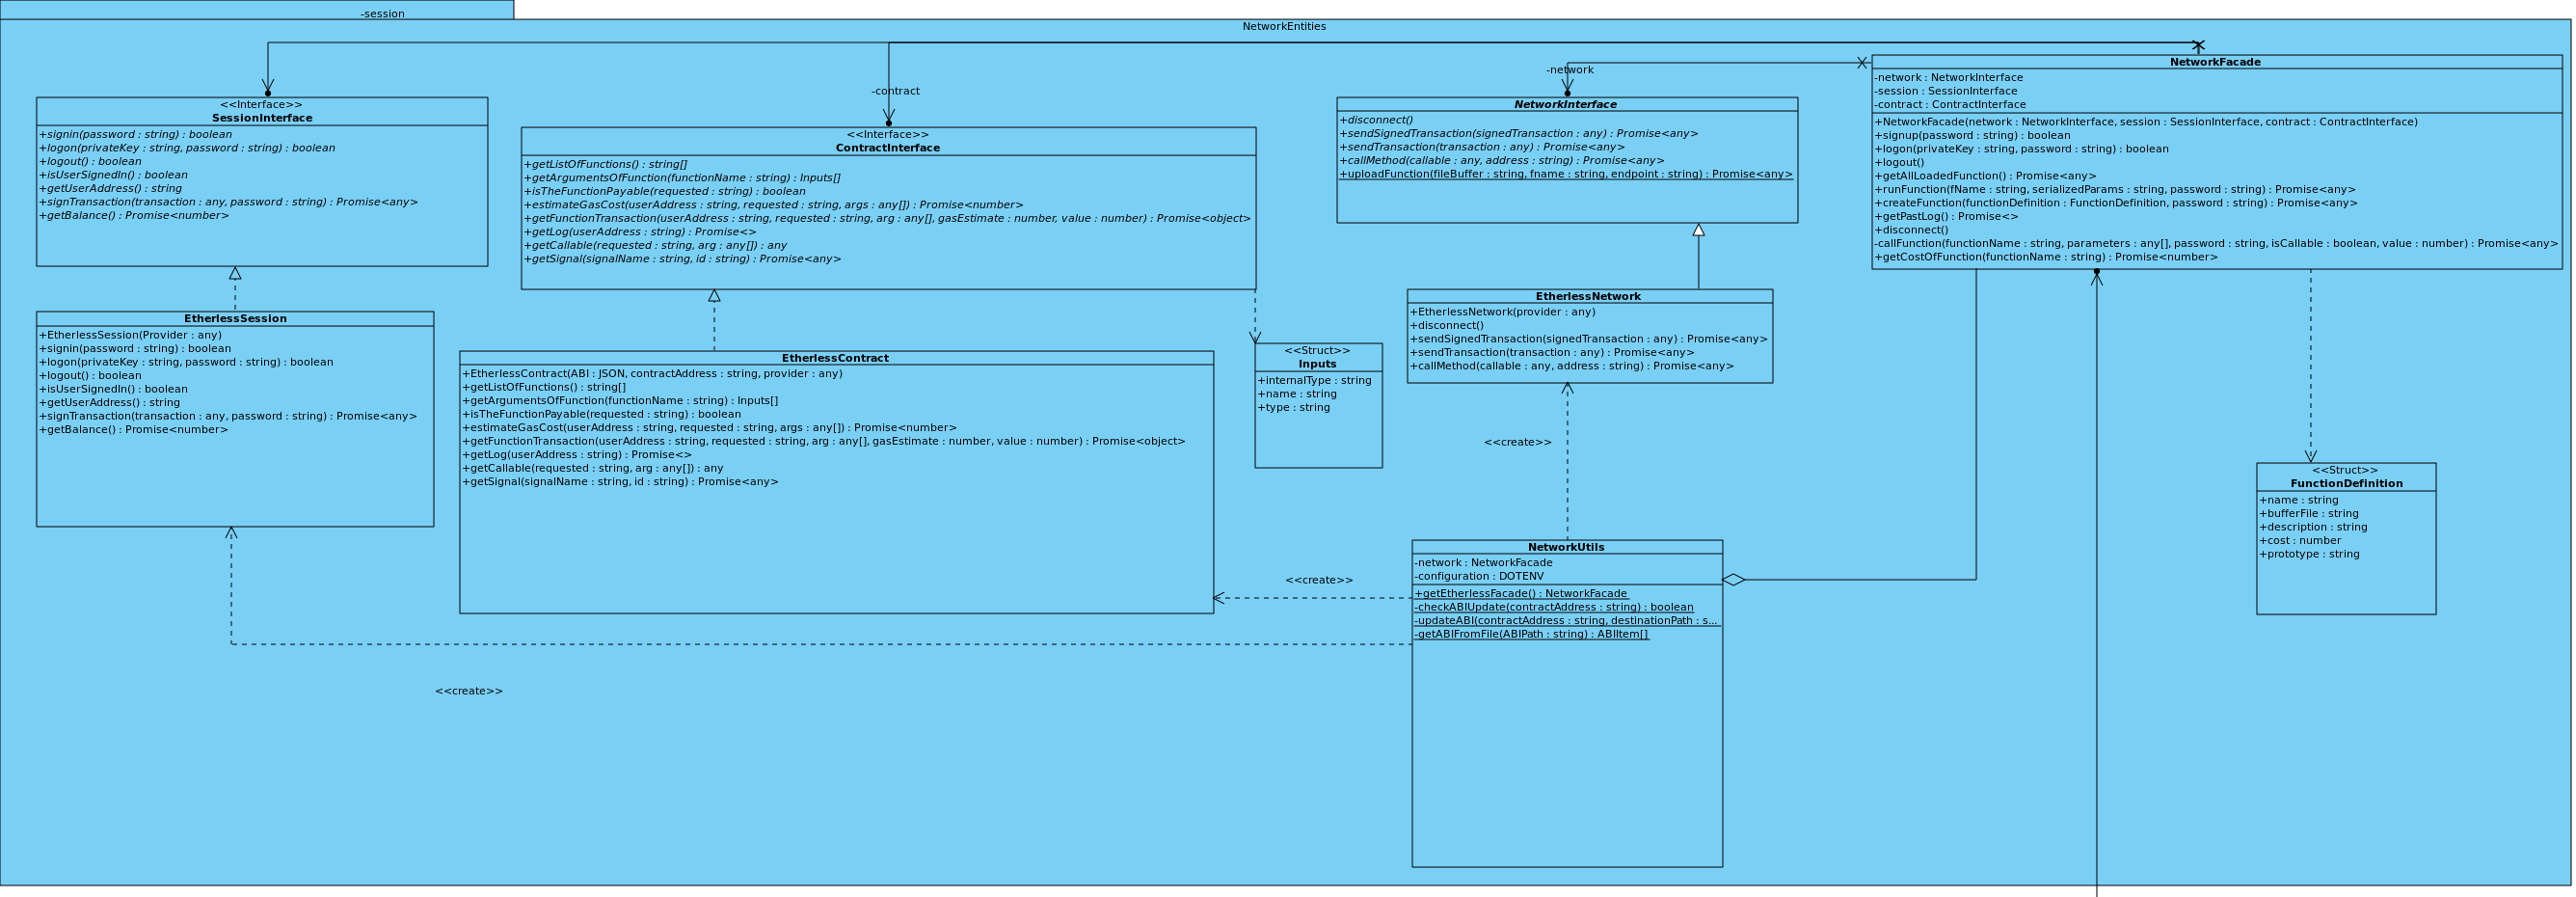
\includegraphics[width=\textwidth]{./res/img/NetworkFacade.png}
	\caption{Architecture overview diagram of Network Entities}
\end{figure}
The Network Entities module is made by:
\begin{itemize}
    \item \textbf{NetworkFacade}: This is the class that defines the main object that the Command Entities interact with, and its the main responsible for communicating with the network;
    \item \textbf{SessionInterface}: This interface defines all the method that every Session object needs to implements to be used in the NetworkFacade, this class include all the method needed to let the user interact with the network ad example login and sign a transaction;
    \item \textbf{ContractInterface}: This interface defines all the method that every Contract object needs to implements to be used in the NetworkFacade, as such as expose the smart contract functionalities and catch signals from it;
    \item \textbf{NetworkInterface}: This abstract class defines the method needed for communication with the Ethereum\glo network and the AWS APIs;
    \item \textbf{NetworkUtils}: This class is a collection of static methods needed for instantiating all the object in NetworkEntities, and keeps all the instances single and defined.
\end{itemize}
The Network Entities module should not expose the constructor of any classes.
The correct way to interact and instantiate the NetworkFacade class is through the static method getNetworkFacadeInstance from NetworkUtils,
this method instantiates our implementation of SessionInterface, ContractInterface, NetworkInterface, and uses them to instantiate the network facade.
\subsubsection{Pros}
This architecture has a good separation of external behavior and internal implementation,
allowing the developers to use any Ethereum\glo network library, creating independence between every component.
\subsubsection{Cons}
This architecture has one major downside, it is difficult to add functionalities without accessing the NetworkFacade and the etherlessContract; We should consider the use of the \textbf{command design pattern} to solve this issue.
Another disadvantage is that if a new developer need a new functionality from any of the interfaces every implementation should reflect the new definition.
\subsubsection{Methods}
\paragraph{NetworkFacade}
\begin{itemize}
    \item \textbf{signup}: registers a new user on the system;
    \item \textbf{logon}: logs in a new user; 
    \item \textbf{logout}: logs out of the system currently logged user;
	\item \textbf{getAllLoadedFunction}: returns the list of all available contract methods;
    \item \textbf{callFunction}: calls the methods of the etherless-smart component; all requests to the smart contract goes through this method;
    \item \textbf{runFunction}: requests execution of a remote function;
    \item \textbf{createFunction}: uploads on the AWS endpoint the required function and register it on the eth network through the etherless-smart component;
    \item \textbf{getPatLog}: return a list of past actions taken by the user;
    \item \textbf{getCostOfFunction}: retrieves from the smart contract the cost of a specific function loaded on the service;
    \item \textbf{disconnect}: disconnects the application from the network.
\end{itemize}
\paragraph{SessionInterface}
\begin{itemize}
    \item \textbf{signup}: provides the signup procedure;
    \item \textbf{logon}: provides the logon procedure using already existing credentials;
    \item \textbf{logout}: discards the credentials by logging out the current user;
    \item \textbf{signTransaction}: signs the provided transaction with logged user account;
    \item \textbf{isUserSignedIn}: checks if there is a singed in user;
    \item \textbf{getUserAddress}: retrieves the user address;
    \item \textbf{getBalance}:retrieves the balance of the logged in user account.
\end{itemize}
\paragraph{ContractInterface}
\begin{itemize}
    \item \textbf{getListOfFunctions}: retrieves all the available contract's methods;
    \item \textbf{getArgumentsOfFunction}: returns all the parameter required to run the requested contract method;
    \item \textbf{isTheFunctionPayable}: returns weather a contract method is needs to receive ethers or not;
    \item \textbf{estimateGasCost}: returns an estimate of how much gas is needed to perform a contract method call;
    \item \textbf{getFunctionTransaction}: builds a transaction object related to a contract method call;
    \item \textbf{getLog}: returns past actions of the given eth account; 
    \item \textbf{getCallable}: maps a contract method name to a its callable form through the network;
    \item \textbf{getSignal}: start listening for a network event.
\end{itemize}
\paragraph{NetworkInterface}
\begin{itemize}
    \item \textbf{getListOfFunctions}: retrieves all the available contract's methods;
    \item \textbf{getArgumentsOfFunction}: returns all the parameter required to run the requested function.
\end{itemize}
\paragraph{NetworkUtils}
\begin{itemize}
    \item \textbf{getEtherlessFacade:}: returns a shared instance of the network interface;
    \item \textbf{checkABIUpdate}: returns weather there is the need of updating smart contract ABI;
    \item \textbf{updateABI}: gets an updated copy of the contract ABI from a remote source;
    \item \textbf{getABIFromFile}: returns a contract ABI retrieved from a local file.
\end{itemize}
\newpage
\subsection{Command Entities}
We base the CommandEntities component on the Command abstract class that is a kind of command design pattern, this means that to add any command to the CLI\glo the developer needs to extend the Command class and implements the exec method.
The Command's constructor exposes the dependency from NetworkFacade using this kind of approach lets us work with mocks and separate the two components of the CLI\glo.
\subsubsection{Architecture overview}
\begin{figure}[h]
	\centering
	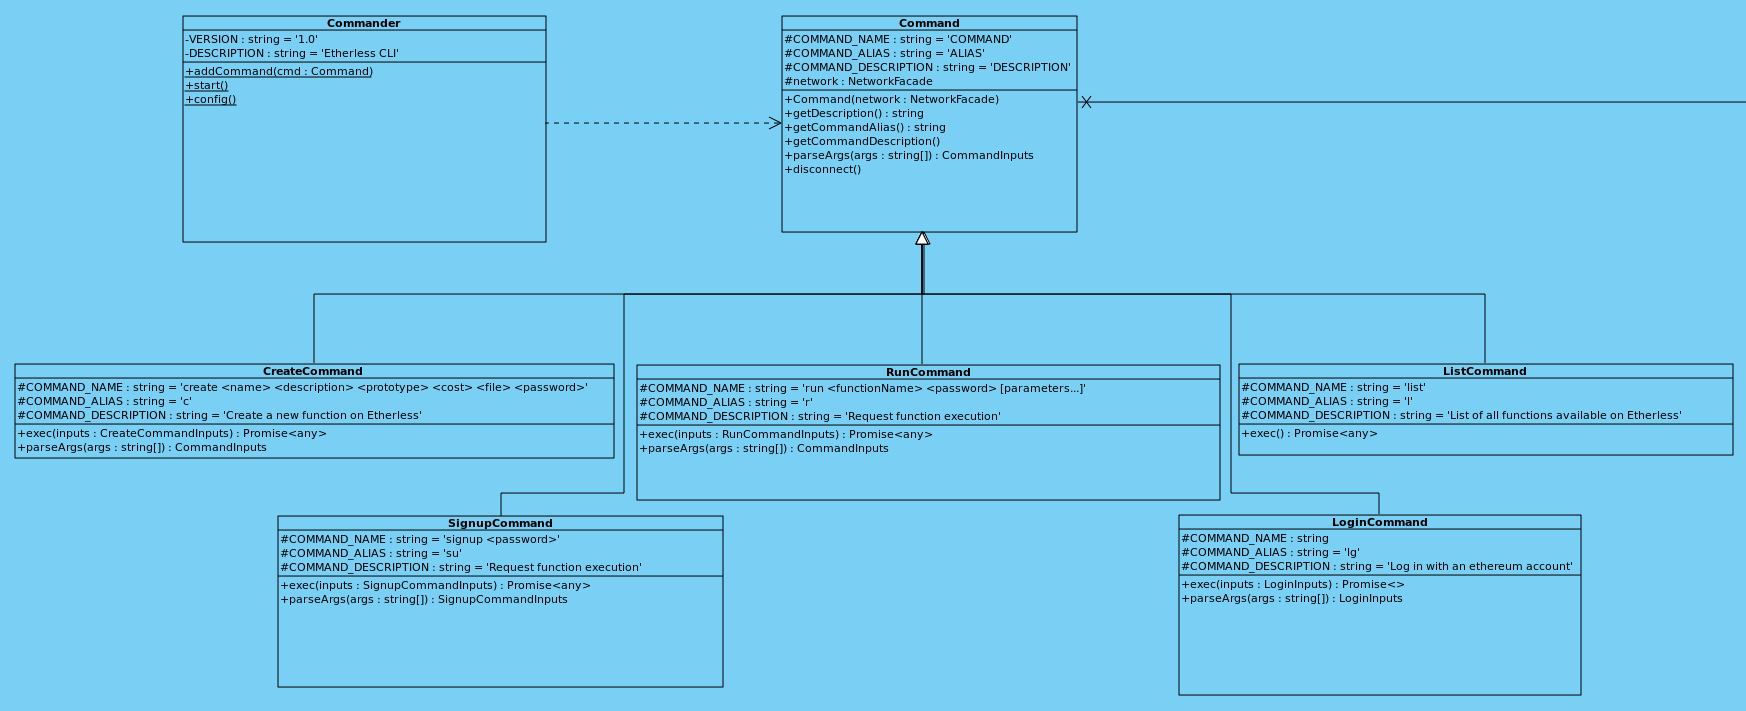
\includegraphics[width=\textwidth]{./res/img/CommandEntities.png}
	\caption{Architecture overview diagram of Command Entities}
\end{figure}
\noindent The Command Entities modules is made by:
\begin{itemize}
    \item \textbf{Command}: This is the main class that all *Command Class should extend because defines the base behavior of every command class;
    \item \textbf{Commander}: This class is a collection of static methods needed to interact with the external library Commander and wraps it, exposing functionalities for adding a new command in the available one.
\end{itemize}
We implemented the basic command functionalities, extending the class abstract class Command:
\begin{itemize}
    \item \textbf{SignUpCommand}: This class implements the sign-up command and allows the user to interact with the Ethereum\glo network for the creation of a new user;
    \item \textbf{LogonCommand}: This class implements the logon command and allows the user to save his credential and use his already existing account;
    \item \textbf{LogoutCommand}: This class implements the logout command and allows the user to delete hid credential;
    \item \textbf{ListCommand}: This class implements the list command and allows the user to interrogate the smart contract and read the list of deployed function;
    \item \textbf{CreateCommand}: This class implements the create command and allows the user to upload in the system a new function to be executed through our service;
    \item \textbf{RunCommand}:This class implements the run command and allows the user to run a deployed function through our service, and moves the credit from his account to our and the function owner.
\end{itemize}
\subsubsection{Pros}
This architecture has good expandability about the functionalities because if a developer wants to add a new function should only extend the command class and insert it in the list of function.
\subsubsection{Cons}
The way we used to instantiate all the classes is not elegant, because we use a method that reads from a list of all the classes that need to instantiate.

\subsubsection{Methods}
\paragraph{Commander}
\begin{itemize}
    \item \textbf{addCommand}: adds a command to the list of available CLI\glo commands;
    \item \textbf{start}: starts processing command input args;
    \item \textbf{start}: sets default CLI\glo information.
\end{itemize}
\paragraph{Command}
\begin{itemize}
    \item \textbf{getDescription}: returns the command description;
    \item \textbf{getCommandAlias}: returns the command alias for the CLI\glo;
    \item \textbf{getCommandsDescriptor}: returns command format for the CLI\glo;
    \item \textbf{parseArgs}: maps CLI\glo inputs to a command-specific inputs data structure;
    \item \textbf{exec}: command execution.
\end{itemize}
